%% (Master) Thesis template
% Template version used: v1.4
%
% Largely adapted from Adrian Nievergelt's template for the ADPS
% (lecture notes) project.


%% We use the memoir class because it offers a many easy to use features.
\documentclass[11pt,a4paper,titlepage]{memoir}

%% Packages
%% ========

%% LaTeX Font encoding -- DO NOT CHANGE
\usepackage[OT1]{fontenc}

%% Babel provides support for languages.  'english' uses British
%% English hyphenation and text snippets like "Figure" and
%% "Theorem". Use the option 'ngerman' if your document is in German.
%% Use 'american' for American English.  Note that if you change this,
%% the next LaTeX run may show spurious errors.  Simply run it again.
%% If they persist, remove the .aux file and try again.
\usepackage[english]{babel}

%% Input encoding 'utf8'. In some cases you might need 'utf8x' for
%% extra symbols. Not all editors, especially on Windows, are UTF-8
%% capable, so you may want to use 'latin1' instead.
\usepackage[utf8]{inputenc}

%% This changes default fonts for both text and math mode to use Herman Zapfs
%% excellent Palatino font.  Do not change this.
\usepackage[sc]{mathpazo}

%% The AMS-LaTeX extensions for mathematical typesetting.  Do not
%% remove.
\usepackage{amsmath,amssymb,amsfonts,mathrsfs}

%% NTheorem is a reimplementation of the AMS Theorem package. This
%% will allow us to typeset theorems like examples, proofs and
%% similar.  Do not remove.
%% NOTE: Must be loaded AFTER amsmath, or the \qed placement will
%% break
\usepackage[amsmath,thmmarks]{ntheorem}

%% LaTeX' own graphics handling
\usepackage{graphicx}

%% We unfortunately need this for the Rules chapter.  Remove it
%% afterwards; or at least NEVER use its underlining features.
\usepackage{soul}

%% This allows you to add .pdf files. It is used to add the
%% declaration of originality.
\usepackage{pdfpages}

%% Some more packages that you may want to use.  Have a look at the
%% file, and consult the package docs for each.
%% See the TeXed file for more explanations

%% [OPT] Multi-rowed cells in tabulars
%\usepackage{multirow}

%% [REC] Intelligent cross reference package. This allows for nice
%% combined references that include the reference and a hint to where
%% to look for it.
\usepackage{varioref}

%% [OPT] Easily changeable quotes with \enquote{Text}
%\usepackage[german=swiss]{csquotes}

%% [REC] Format dates and time depending on locale
\usepackage{datetime}

%% [OPT] Provides a \cancel{} command to stroke through mathematics.
%\usepackage{cancel}

%% [NEED] This allows for additional typesetting tools in mathmode.
%% See its excellent documentation.
\usepackage{mathtools}

%% [ADV] Conditional commands
%\usepackage{ifthen}

%% [OPT] Manual large braces or other delimiters.
%\usepackage{bigdelim, bigstrut}

%% [REC] Alternate vector arrows. Use the command \vv{} to get scaled
%% vector arrows.
%% \usepackage[h]{esvect}

%% [NEED] Some extensions to tabulars and array environments.
\usepackage{array}

%% [OPT] Postscript support via pstricks graphics package. Very
%% diverse applications.
%\usepackage{pstricks,pst-all}

%% [?] This seems to allow us to define some additional counters.
%\usepackage{etex}

%% [ADV] XY-Pic to typeset some matrix-style graphics
%\usepackage[all]{xy}

%% [OPT] This is needed to generate an index at the end of the
%% document.
%\usepackage{makeidx}

%% [OPT] Fancy package for source code listings.  The template text
%% needs it for some LaTeX snippets; remove/adapt the \lstset when you
%% remove the template content.
\usepackage{listings}
\lstset{language=TeX,basicstyle={\normalfont\ttfamily}}

%% [REC] Fancy character protrusion.  Must be loaded after all fonts.
\usepackage[activate]{pdfcprot}

%% [REC] Nicer tables.  Read the excellent documentation.
\usepackage{booktabs}


%% Our layout configuration.  DO NOT CHANGE.
%% Memoir layout setup

%% NOTE: You are strongly advised not to change any of them unless you
%% know what you are doing.  These settings strongly interact in the
%% final look of the document.

% Dependencies
\usepackage{ETHlogo}

% Turn extra space before chapter headings off.
\setlength{\beforechapskip}{0pt}

\nonzeroparskip
\parindent=0pt
\defaultlists

% Chapter style redefinition
\makeatletter

\if@twoside
  \pagestyle{Ruled}
  \copypagestyle{chapter}{Ruled}
\else
  \pagestyle{ruled}
  \copypagestyle{chapter}{ruled}
\fi
\makeoddhead{chapter}{}{}{}
\makeevenhead{chapter}{}{}{}
\makeheadrule{chapter}{\textwidth}{0pt}
\copypagestyle{abstract}{empty}

\makechapterstyle{bianchimod}{%
  \chapterstyle{default}
  \renewcommand*{\chapnamefont}{\normalfont\Large\sffamily}
  \renewcommand*{\chapnumfont}{\normalfont\Large\sffamily}
  \renewcommand*{\printchaptername}{%
    \chapnamefont\centering\@chapapp}
  \renewcommand*{\printchapternum}{\chapnumfont {\thechapter}}
  \renewcommand*{\chaptitlefont}{\normalfont\huge\sffamily}
  \renewcommand*{\printchaptertitle}[1]{%
    \hrule\vskip\onelineskip \centering \chaptitlefont\textbf{\vphantom{gyM}##1}\par}
  \renewcommand*{\afterchaptertitle}{\vskip\onelineskip \hrule\vskip
    \afterchapskip}
  \renewcommand*{\printchapternonum}{%
    \vphantom{\chapnumfont {9}}\afterchapternum}}

% Use the newly defined style
\chapterstyle{bianchimod}

\setsecheadstyle{\Large\bfseries\sffamily}
\setsubsecheadstyle{\large\bfseries\sffamily}
\setsubsubsecheadstyle{\bfseries\sffamily}
\setparaheadstyle{\normalsize\bfseries\sffamily}
\setsubparaheadstyle{\normalsize\itshape\sffamily}
\setsubparaindent{0pt}

% Set captions to a more separated style for clearness
\captionnamefont{\sffamily\bfseries\footnotesize}
\captiontitlefont{\sffamily\footnotesize}
\setlength{\intextsep}{16pt}
\setlength{\belowcaptionskip}{1pt}

% Set section and TOC numbering depth to subsection
\setsecnumdepth{subsection}
\settocdepth{subsection}

%% Titlepage adjustments
\pretitle{\vspace{0pt plus 0.7fill}\begin{center}\HUGE\sffamily\bfseries}
\posttitle{\end{center}\par}
\preauthor{\par\begin{center}\let\and\\\Large\sffamily}
\postauthor{\end{center}}
\predate{\par\begin{center}\Large\sffamily}
\postdate{\end{center}}

\def\@advisors{}
\newcommand{\advisors}[1]{\def\@advisors{#1}}
\def\@department{}
\newcommand{\department}[1]{\def\@department{#1}}
\def\@thesistype{}
\newcommand{\thesistype}[1]{\def\@thesistype{#1}}

\renewcommand{\maketitlehooka}{\noindent\ETHlogo[2in]}

\renewcommand{\maketitlehookb}{\vspace{1in}%
  \par\begin{center}\Large\sffamily\@thesistype\end{center}}

\renewcommand{\maketitlehookd}{%
  \vfill\par
  \begin{flushright}
    \sffamily
    \@advisors\par
    \@department, ETH Z\"urich
  \end{flushright}
}

\checkandfixthelayout

\setlength{\droptitle}{-48pt}

\makeatother

% This defines how theorems should look. Best leave as is.
\theoremstyle{plain}
\setlength\theorempostskipamount{0pt}

%%% Local Variables:
%%% mode: latex
%%% TeX-master: "thesis"
%%% End:


%% Theorem environments.  You will have to adapt this for a German
%% thesis.
%% Theorem-like environments

%% This can be changed according to language. You can comment out the ones you
%% don't need.

\numberwithin{equation}{chapter}

%% German theorems
%\newtheorem{satz}{Satz}[chapter]
%\newtheorem{beispiel}[satz]{Beispiel}
%\newtheorem{bemerkung}[satz]{Bemerkung}
%\newtheorem{korrolar}[satz]{Korrolar}
%\newtheorem{definition}[satz]{Definition}
%\newtheorem{lemma}[satz]{Lemma}
%\newtheorem{proposition}[satz]{Proposition}

%% English variants
\newtheorem{theorem}{Theorem}[chapter]
\newtheorem{example}[theorem]{Example}
\newtheorem{remark}[theorem]{Remark}
\newtheorem{corollary}[theorem]{Corollary}
\newtheorem{definition}[theorem]{Definition}
\newtheorem{lemma}[theorem]{Lemma}
\newtheorem{proposition}[theorem]{Proposition}

%% Proof environment with a small square as a "qed" symbol
\theoremstyle{nonumberplain}
\theorembodyfont{\normalfont}
\theoremsymbol{\ensuremath{\square}}
\newtheorem{proof}{Proof}
%\newtheorem{beweis}{Beweis}


%% Helpful macros.
%% Custom commands
%% ===============

%% Special characters for number sets, e.g. real or complex numbers.
\newcommand{\C}{\mathbb{C}}
\newcommand{\K}{\mathbb{K}}
\newcommand{\N}{\mathbb{N}}
\newcommand{\Q}{\mathbb{Q}}
\newcommand{\R}{\mathbb{R}}
\newcommand{\Z}{\mathbb{Z}}
\newcommand{\X}{\mathbb{X}}

%% Fixed/scaling delimiter examples (see mathtools documentation)
\DeclarePairedDelimiter\abs{\lvert}{\rvert}
\DeclarePairedDelimiter\norm{\lVert}{\rVert}

%% Use the alternative epsilon per default and define the old one as \oldepsilon
\let\oldepsilon\epsilon
\renewcommand{\epsilon}{\ensuremath\varepsilon}

%% Also set the alternate phi as default.
\let\oldphi\phi
\renewcommand{\phi}{\ensuremath{\varphi}}


\usepackage{todonotes}
\usepackage{float}
\usepackage{caption}
\graphicspath {{sequence-diagrams/}, {illustrations/}, {plots/}}
\usepackage{rotating}
\usepackage{listings}
\usepackage{xcolor}
\usepackage{booktabs}

\definecolor{codegreen}{rgb}{0,0.6,0}
\definecolor{codegray}{rgb}{0.5,0.5,0.5}
\definecolor{codepurple}{rgb}{0.58,0,0.82}
\definecolor{backcolour}{rgb}{0.95,0.95,0.92}
 
\lstdefinestyle{mystyle}{
    backgroundcolor=\color{backcolour},   
    commentstyle=\color{codegreen},
    keywordstyle=\color{magenta},
    numberstyle=\tiny\color{codegray},
    stringstyle=\color{codepurple},
    basicstyle=\ttfamily\footnotesize,
    breakatwhitespace=false,         
    breaklines=true,                 
    captionpos=b,                    
    keepspaces=true,                 
    numbers=left,                    
    numbersep=5pt,                  
    showspaces=false,                
    showstringspaces=false,
    showtabs=false,                  
    tabsize=2
}
 
\lstset{style=mystyle}

%% Make document internal hyperlinks wherever possible. (TOC, references)
%% This MUST be loaded after varioref, which is loaded in 'extrapackages'
%% above.  We just load it last to be safe.
\usepackage[linkcolor=black,colorlinks=true,citecolor=black,filecolor=black]{hyperref}

\usepackage[masterthesis]{systems-cover/systems-cover}
\covernum{265}
\covertitle{Improving Session-Based Recommendation Systems with Item Embeddings}
\coverauthor{Mohammed Ajil}
\coverdate{September 13, 2019}
\coversupervisedby{Bojan Karlas, Ce Zhang}
\coverincollaboration{Digitec Galaxus AG}

%% Document information
%% ====================

\title{Improving Session-Based Recommendation Systems with Item Embeddings}
\author{Mohammed Ajil}
\thesistype{Master Thesis}
\advisors{Advisors: Prof.\ Ce Zhang, Bojan Karlas}
\department{Department of Computer Science}
\date{September 13, 2019}

\begin{document}

\frontmatter

%% Title page is autogenerated from document information above.  DO
%% NOT CHANGE.
\begin{titlingpage}
  \calccentering{\unitlength}
  \begin{adjustwidth*}{\unitlength-24pt}{-\unitlength-24pt}
    \maketitle
  \end{adjustwidth*}
\end{titlingpage}

%% The abstract of your thesis.  Edit the file as needed.
\begin{abstract}
  This work examines how a session-based recommendation system can be combined with pre-trained item embeddings.
  Session-based recommendation systems are highly relevant in online services such as music or video streaming services and e-commerce, more and more so when the item catalogs grow into the millions.
  The approach presented in this work is tested in a production setting with live users, using a industry dataset magnitudes larger than the datasets used in works this thesis is based on.
  We show that session-recommendation performs better than classical recommendation approaches, however the combination of the two approaches was unsuccessful, failing primarily because of the Long Tail phenomenon. 
\end{abstract}


%% TOC with the proper setup, do not change.
\cleartorecto
\tableofcontents
\mainmatter
%% Your real content!
\chapter{Introduction}
Recommendation systems are a field in machine learning that get more and more attention.
The most general definition of a recommendation system is a system that aids a user in some kind of decision process.
Usually a very large number of choices is available in such a decision process, such as which music to listen to from a selection of millions of tracks, or which products to buy from a catalog of millions of products.
Depending on the recommendation system, information about the items, about the users, and about the interaction of users with items is taken into account.
\par
The first approaches to recommendation engines mainly used interaction data, since the tools available at that time did not allow for an incorporation of image, text, or side-information.
In recent years deep neural networks enabled the use of more types of datapoints, such as images and text for example.
Further recurrent neural networks allowed to explicitly model sequence data, which opened up many possibilities in this space, since users tend to change over time.
Specifically GRU4Rec (c.f.~\cite{gru4rec}) gained attention as an RNN based approach to model session data.
In this setting we try to model the sequence of events a user makes when he browses some catalog, instead of just static information about items and users.
Another advantage would be that in a session-based approach the identification of the user is not necessary, because identifying users is a difficult task in itself.
Since the session serves as a basis for recommendations, the user can be used to additionally improve the results, but is not necessary for a recommendation.
This is in contrast to other methods such as collaborative filtering where the user must be known.
In~\cite{hierarchical} a model is proposed that does exactly that, it uses GRU4Rec as a basis and extends it with a user-level representation.
\par
As mentioned before DNNs have allowed the ingestion of other types of datapoints.
This allows the vectorization of structured data, such as representing items in a euclidian vector space.
The advantage of this is that the abstract concept of similarity of items can be quantified.
This allows to better understand and navigate a large catalog of items.
The authors of~\cite{meta_prod2vec} introduced a model that can just do that.
By injesting session based data about the items, as well as categorical side information the model fits a fixed sized vector in an euclidian space for each item.
This model fits these vectors such that the similar items receive a similar representation.
\par
The goal of this work is to explore the possibility of combining the two concepts such that a session-based recommendation system can make use of the quantifiable similarity between items.
\chapter{Background}

\section{Recommendation Systems}
\subsection{Problem Statement}
\subsection{Variants}
\subsection{Well-Known Systems}
\begin{itemize}
\item Specify the Problem of Recommendation as a scoring problem on items
\item Describe possile bases for recommendation (User Based, Item Based, Session Based)
\item Describe most popular existing solutions (Collaborative Filtering, Wide and Deep Learning)
\end{itemize}

\section{Concepts/Models/...}
\subsection{Recurrent Neural Networks}
\subsection{Generative Adversarial Network Framework}
\subsection{Hierarchical RNNs for personalized Recommendations}
\cite{hierarchical}
\subsection{Professor Forcing}
\cite{profforce}
\subsection{Meta-Prod2Vec}
\cite{prod2vec}
\begin{itemize}
\item Describe RNNs
\item Describe Hiearchical RNNs
\item Describe the GAN Framework
\item Describe Professor Forcing as an application of the GAN Framework to RNNs
\item Describe Meta-Prod2Vec as an embedding framework and where we would use it inside our model
\end{itemize}

\section{KPIs}
\subsection{Click-Through-Rate}
\subsection{Conversion Rate}
\begin{itemize}
\item Describe different KPIs
\item What do they meaure, how to optimize for it
\end{itemize}
\chapter{Dataset}

\section{Data Collection}
In this work we will use the data generated by the tracking systems of Digitec Galaxus AG.
The following sequence-diagram gives an overview of the data collection process.

\begin{figure}[H]
	\centering
	\captionsetup{width=0.8\textwidth}
    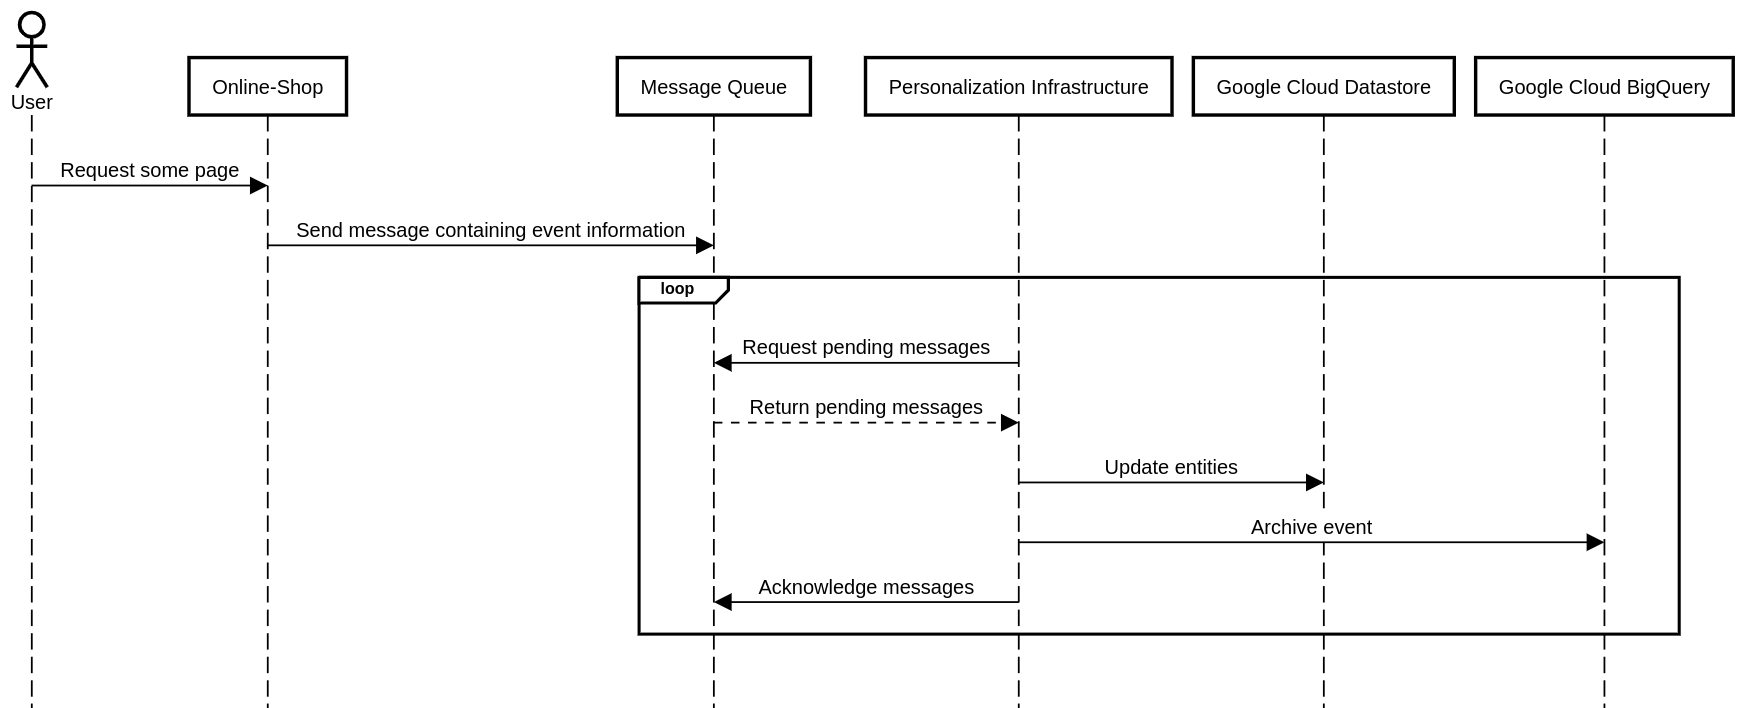
\includegraphics[width=\textwidth]{collecting-data.png}
    \caption{Collecting user interaction data on digitec.ch and galaxus.ch}
    \label{fig:collecting_data}
\end{figure}

When a user requests a specific page, the Online-Shop Application will collect some information on the user such as UserId, requested page, User Agent etc.
This information is packaged as a message representing this specific event and then sent to a message queue.
After that the Personalization Infrastructure will process these events by requesting batches of unprocessed messages.
For each event then the Personalization Infrastructure will do two things: First it will update the involved entities, second it will archive the event.
In the former case a managed Key-Value store (Google Cloud Datastore) is used to store entities.
Examples of such entities are Shopping Carts, Orders, and Last Viewed Products.
In principle these entities represent the current state of various entities appearing in the context of the Online-Shop.
In the latter case a managed Data Warehousing solution (Google BigQuery) is used, this solution provides the possibility to store large amounts of data in append-only tables.
The data stored there is mainly denormalized, such that easy extraction is possible.
Each row in these append-only tables contains all information belonging to a single event produced by a user.
Essentially the data stored in the Key-Value store is the sum of all events stored in the data warehouse.

\section{Data Preparation}
To be able to focus on the model implementation when implementing the model we want to prepare the data for congestion as far as possible.
Therefore the extraction and preparation of the dataset is implemented separately from the model implementation.
The process is very similary to the process described in~\cite{hierarchical}.
\paragraph{Data Extraction}
In the first step we extract the raw data from the data warehouse, selecting the following pieces of information: ProductId, LastLoggedInUserId, UserId, SessionId, User Agent, Timestamp.
Most of the properties are self-explanatory, except LastLoggedInUserId.
This property represents the UserId last seen on a specific device accessing the Online-Shop, therefore it is useful if the user did not actively log in to the account.
In this case we would not know which user accessed the page, however using this property we can complete missing UserIds in the dataset.
The data extracted is limited to the events producted by visiting a product detail page as seen in figure~\ref{fig:product_detail}.
This filtering is done because this work focuses on recommending products, in another setting other data might also be relevant.
The extracted data is stored in several shards of CSV files, each shard approximately represents the events of one day.

\begin{figure}[ht]
	\centering
	\captionsetup{width=0.8\textwidth}
    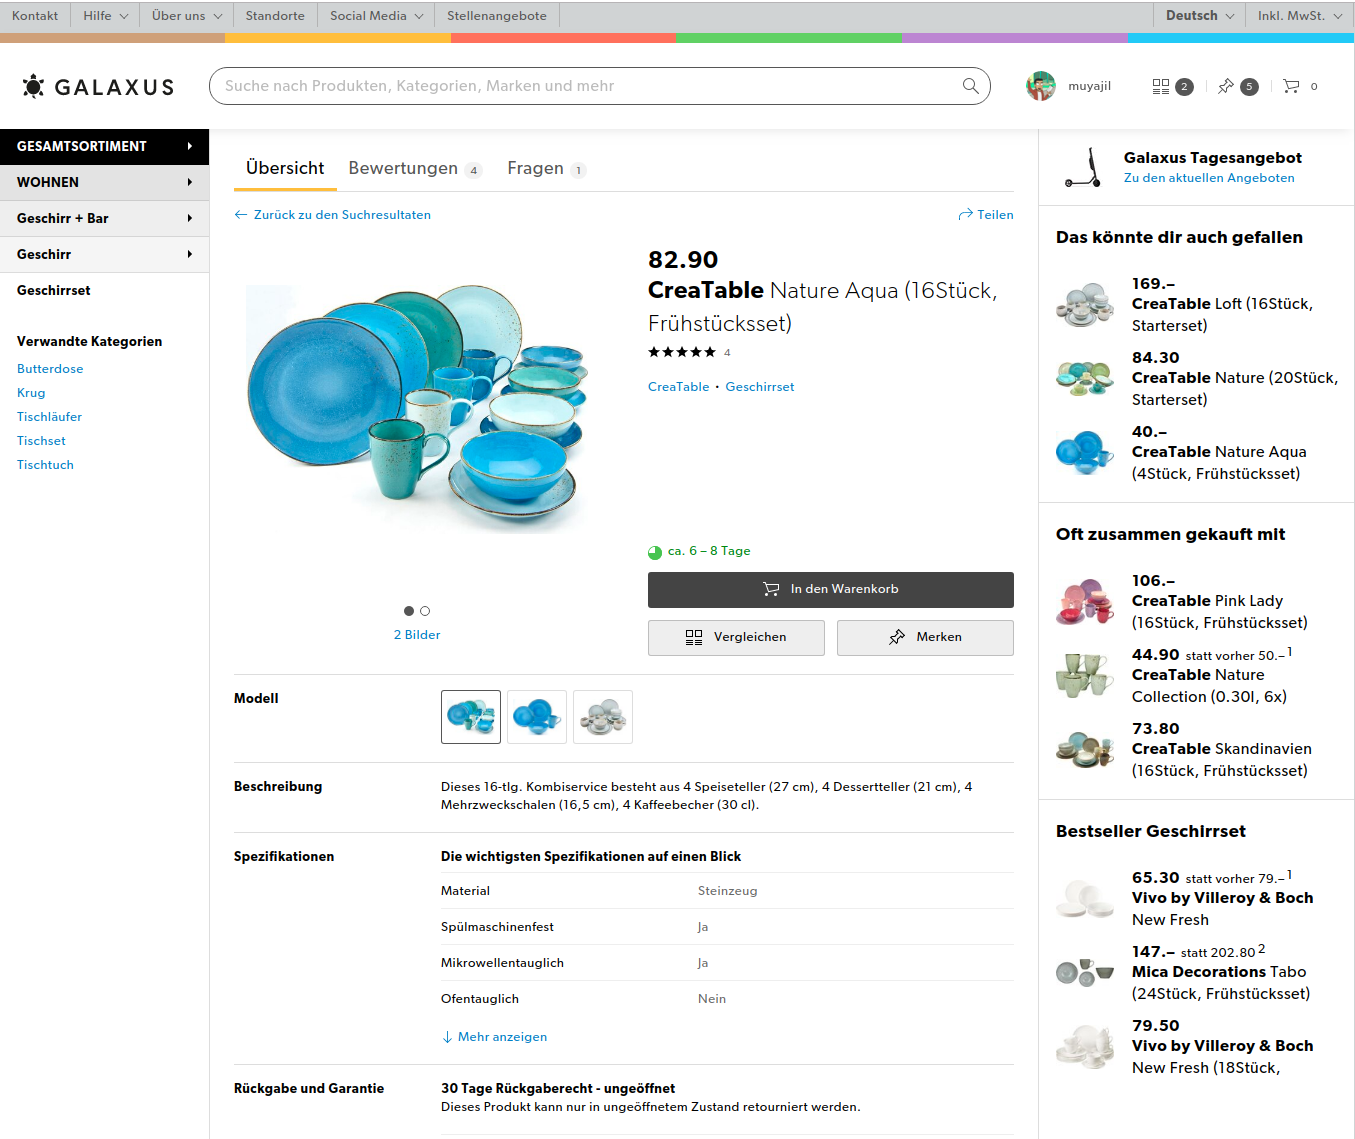
\includegraphics[width=\textwidth]{product-detail.png}
    \caption{Product Detail Page on galaxus.ch}
    \label{fig:product_detail}
\end{figure}

\paragraph{Cleaning data}
In the next step the data is cleaned, which involves mainly two steps.
Anytime we encounter an event where we do not know the user, we try to complete the information with the LastLoggedInUserId. 
If we do not know the LastLoggedInUserId as well we discard the event. \\
There are many well-known bots roaming the Internet collecting various types of information on websites.
Most famously the Google Bot which crawls the content of any website to determine the quality of the site and influence the rank of the website in Google searches.
There are some open-source lists that collect the User Agents of these bots.
The User Agent of a client accessing a website usually describes the type of device used, in the case of "good" bots they explicitly tell the server that the "device" accessing the website is actually a bot.
Using one of these lists\footnote{\url{https://raw.githubusercontent.com/monperrus/crawler-user-agents/master/crawler-user-agents.json}} the events produced by bots are removed from the dataset.
\paragraph{Aggregation of events}
The next step is to aggregate the events on two levels, first grouping events that were generated in the same session and second grouping these sessions by users.
The resulting data structure looks as follows:

\begin{minipage}{\linewidth}
    \begin{lstlisting}[language=Python,frame=single,caption=Data Structure for user-events,label=code:user-events]
    "<UserId_1>": {
        "<SessionId_1>": {
            "StartTime": "<Timestamp of first event>",
            "Events": [
                {
                    "ProductId": "<ProductId_1>",
                    "Timestamp": "<Timestamp_1>"
                },
                {
                    "ProductId": "<ProductId_2>",
                    "Timestamp": "<Timestamp_2>"
                }
            ]
        }
    }
    \end{lstlisting}
\end{minipage}
This is done by processing one shard after another, when a shard is finished the JSON representation of this shard is saved in a separate file.
The reason is that the large amount of datapoints cannot be kept in memory altogether.

\paragraph{Merging shards}
Since the shards only approximate the events of one day, it is not possible to assume that a session is completely represented in one shard, it might be distributed across multiple.
Therefore it is necessary to merge the data in the different shards, however since it is not efficient to keep all the information in one file, a different method of paritioning is needed.
However as we will see later it is further necessary that all the events produced by a single user are in the same file.
An easy way of achieving this is by partitioning by UserId.
Each shard is processed as follows:

\begin{minipage}{\linewidth}
    \begin{lstlisting}[language=Python,frame=single,caption=Merging shards,label=code:merging-shards]
    for shard in shards:
        for i in range(num_target_files):
            relevant_user_ids = list(filter(lambda x: int(x) % num_target_files == i, shard.keys()))
            output_path = merged_shards_prefix + str(i) + '.json'
            output_file = json.load(output_path)
            for user_id in relevant_user_ids:
                for session_id in shard[user_id]:
                    # Merge events from output_file and shard
    \end{lstlisting}
\end{minipage}

\paragraph{Filtering}
Now we have some number of files containing all the information relevant to some users.
As the authors of~\ref{hierarchical} mentioned as well, it makes sense to filter out some datapoints.
Specifically the following:
\begin{itemize}
    \item Remove items with low support (min 5 Events per product)
    \item Remove users with few sessions (min 5 Sessions per user)
    \item Remove sessions with few events (min 3 Events per session)
\end{itemize}
The reasons for removing these is rather obvious.
Items with few interactions are not optimal for modeling, sessions that are too short are not really informative, and finally users with few sessions produce few cross-session information.

\paragraph{Subsampling}
Prototyping models with very large datasets is very inefficient.
Therefore several different sizes of the dataset were produced.
First the approximate number of users and the exact number of products desired in the dataset is defined.
This was done by sampling from the set of products with a probability proportional to the number of events on that product.
In a next step the partitions of the data are processed, iterating through the sessions of the users.
For each sessions we remove the products that were not chosen to be kept, if the session is still long enough, the session is kept.
Further a user is kept in the dataset if the number of filtered sessions is still large enough.
This process is repeated for the different partitions until the number of users is larger than the approximate number of desired users.

\paragraph{Embedding Dictionary}
As we will see in~\ref{model_arch} a version of the model uses one-hot encodings for representing products.
Therefore the product IDs referenced in the dataset need to be mapped into a continuous ID space, otherwise it is not possible to produce one-hot encodings.
The process for this is straight forward: Start with EmbeddingId 0 then iterate through all the sessions, and each time a product is seen for the first time it will be assigned the EmbeddingId and the EmbeddingId is increased by 1.

\section{User Parallel Batches}
Since we are dealing with sequence data, it is not trivial to produce batches for the model to ingest.
Especially since the sequences can have different lengths, and the number of sessions varies from user to user.
User Parallel Batching is a way of having fixed size batches that can be ingested by the model, while allowing for sequences to have different lengths and users to have a different number of sessions.
Usually in these cases the sequences are padded with some neutral value, however in this case there is no neutral product, and the introduction of such a neutral product might influence the results.
Furthermore when processing sequence data it usually means that a datapoint is the input for the next datapoint, which means we still need to have the ordered sequence data.
To illustrate these batches lets assume that there are 4 users with the sessions as in figure~\ref{fig:user_parallel_batches}.

\begin{figure}[h]
	\centering
	\captionsetup{width=0.8\textwidth}
    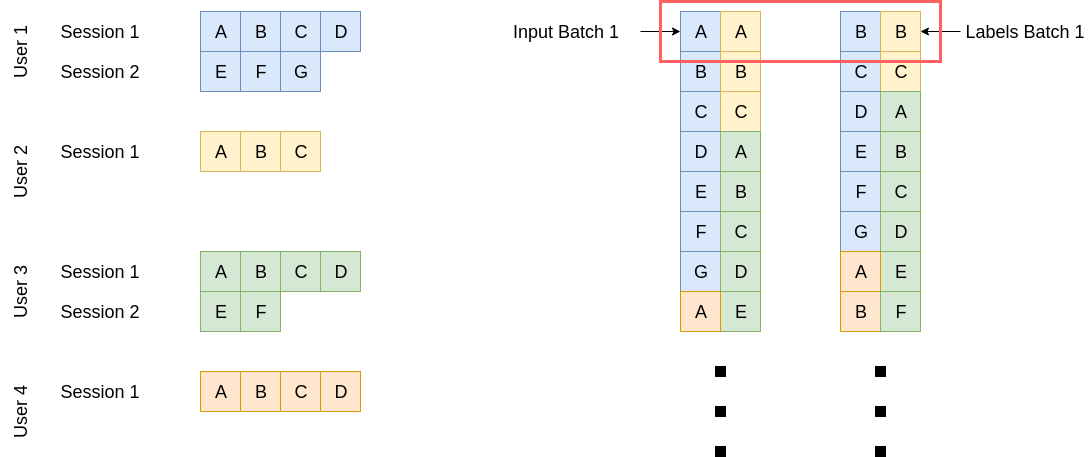
\includegraphics[width=\textwidth]{user_parallel_batches.png}
    \caption{User Parallel Batches}
    \label{fig:user_parallel_batches}
\end{figure}

In principle a batch of size $x$ will contain an event from $x$ different users.
Essentially the labels are the event that happens after the input event.
\\
The data representation shown in listing~\ref{code:user-events} explicitly to enable efficient generation of user parallel batches.

\chapter{System Overview}

\section{Model Architecture}\label{sec:model_arch}
The inspiration from this work comes from~\cite{hierarchical}.
The authors designed a model architecture that can capture 
\begin{itemize}
    \item The architecture builds on what the authors of~\cite{gru4rec} designed.
    \item The model called GRU4Rec uses a RNN using GRUs to model the session data.
    \item The learning task boils down to learn the typical paths users take through the online-store.
    \item This model is not personalized, since we do not use the information which user generated a specific session.
    \item The idea is to predict which product the users wants to see next and provide him or her with a shortcut.
    \item Now we have a fixed size representation of a session.
    \item Now we could try to learn how sessions evolve over time by adding another RNN on the above layer.
    \item This is done by using the session representation as the input, and therefore the hidden state represents the evolvement of the user.
    \item 
    \item Describe how it captures the session representation
    \item illustration for hierarchical neural network
    \item Describe Model Architecture
    \item Describe different Components of Model Architecture
\item Describe different variants of the model (with/without pf, with/without embeddings)
\end{itemize}
\subsection{Model training}
\section{Product Embedding}
\begin{itemize}
    \item We introducted the model architecture for Meta Prod2Vec in~\todo{Add reference to section about metaprod2vec}
    \item We used the features brand, producttype, and price class.
    \item The price class is computed by determining the quantiles of products in the same product type and categorizing the products into 4 price classes.
    \item We used equal weights for all the metadata.
    \item 
    \item 
    \item Write about the features used, what are the transformations etc.
\end{itemize}

\section{Implementation}

\begin{itemize}
    \item we could make a diagram showing the different components
\item Describe Class Diagram
\item Describe prediction mode/training mode
\item Describe problems that arose during training (extensive resources used for so many products and users)
\end{itemize}
\subsection{API}\label{sec:api}
As described above the model is implemented in Tensorflow\footnote{\url{http://tensorflow.org}}.
Tensorflow provides a mechanism to export tensorflow models as so called SavedModel\footnote{\url{https://github.com/tensorflow/tensorflow/blob/master/tensorflow/python/saved_model/README.md}}, which is the way Tensorflow serializes models universally.
They also provide a premade Docker image\footnote{\url{https://hub.docker.com/r/tensorflow/serving}} which allows the model to be served as a REST or GRPC API.
\begin{itemize}
\item Describe API
\end{itemize}

\section{Production Setup}
Digitec Galaxus AG is the largest online-retailer in Switzerland.
They operate galaxus.ch and digitec.ch. The former is a general online-shop comparable to Amazon. 
The latter is specialized in Electronics.
Distributed on the different sections of the site there are several recommendation engines populating the content the users see.
Examples are the landing page\todo{Add screenshot} and multiple engines on the product detail page\todo{Add screenshot}.
% At the time of writing these engines were either recommending products or marketing pages. 
% \par
% Marketing Pages are a part of Digitec Galaxus' marketing strategy.
% There is a editorial team which is separated by a chinese wall from the product departement.
% This team writes independant reviews and other stories including current news.
% These pages give the customers a second reason to interact with the platform, by establishing themselves as a news platform for users.
% Therefore it makes sense to invest in recommendations of articles, since this allows the user to be familiar with the platform, and later preferring it for an online purchase.
% These pages are not considered in this work, however the model should be applicable to marketing pages as well. 

% \subsection{Survival of the Fittest Framework}
% As mentioned above there are multiple locations, such as the product detail page, in which recommendation engines can display content.
% Moreover in each of these locations is it possible to have multiple spots which display content from recommendation engines.
% For example on the product detail page there are multple spots displaying recommendations.
% The Survival of the Fittest Framework is a system designed to decide which recommendation engine runs in which spot. \todo{Show an illustration for the framework}
% The framework is a way of tackling the exploration exploitation tradeoff.
% The definition which recommendation engine is allowed to be displayed in which spot is done manually, since not all combinations of the two make sense from a user experience perspective.
% In principle popular recommendation engines get a proportionally higher probability to be selected when such a page is accessed by a specific user, while maintaining some restrictions.
% This probability of being selected is defined as follows:\todo{Add specific formula}
% \[
%     p_{xij} = max(0.05, )
% \]
% Where $p_{xij}$ is the probability of recommendation engine $x$ being displayed on location $i$ and spot $j$.
% This probability is computed constantly, automatically based on a stream of user clicks.
% The Click-Through-Rate is the relevant metric for this computation because as described in~\ref{conversion_rate} this can only be estimated from the sales, since the true intent of the user cannot be reliably identified.
% Therefore less popular or new recommendation engines still can be selected to be displayed, allowing for exploration of different approaches.
% Should an engine become popular due to an improvement in the logic behind it, the probability of display increases automatically as more users interact with this element.

There is a framework that computes probabilities which specific recommendation engine provides the content for a specific location.
Further the framework then chooses the content for each location based on the probabilities computed before and some other constraints such as minimum and maximum value.
However to test the model implemented in this work this framework is bypassed by a A/B Testing engine, therefore this framework is not part of this work.
The specific tests and the test setup is described in~\ref{sec:exp_setup}, for the understanding of the following it is enough to assume that some independant system is providing recommendation requests to the recommendation system.
Using the API containers described in~\ref{sec:api} we can serve these requests.
The sequence-diagram in figure~\ref{fig:serving_recs} should give an overview on how the system is integrated in the production environment.

\begin{figure}[H]
	\centering
	\captionsetup{width=0.8\textwidth}
    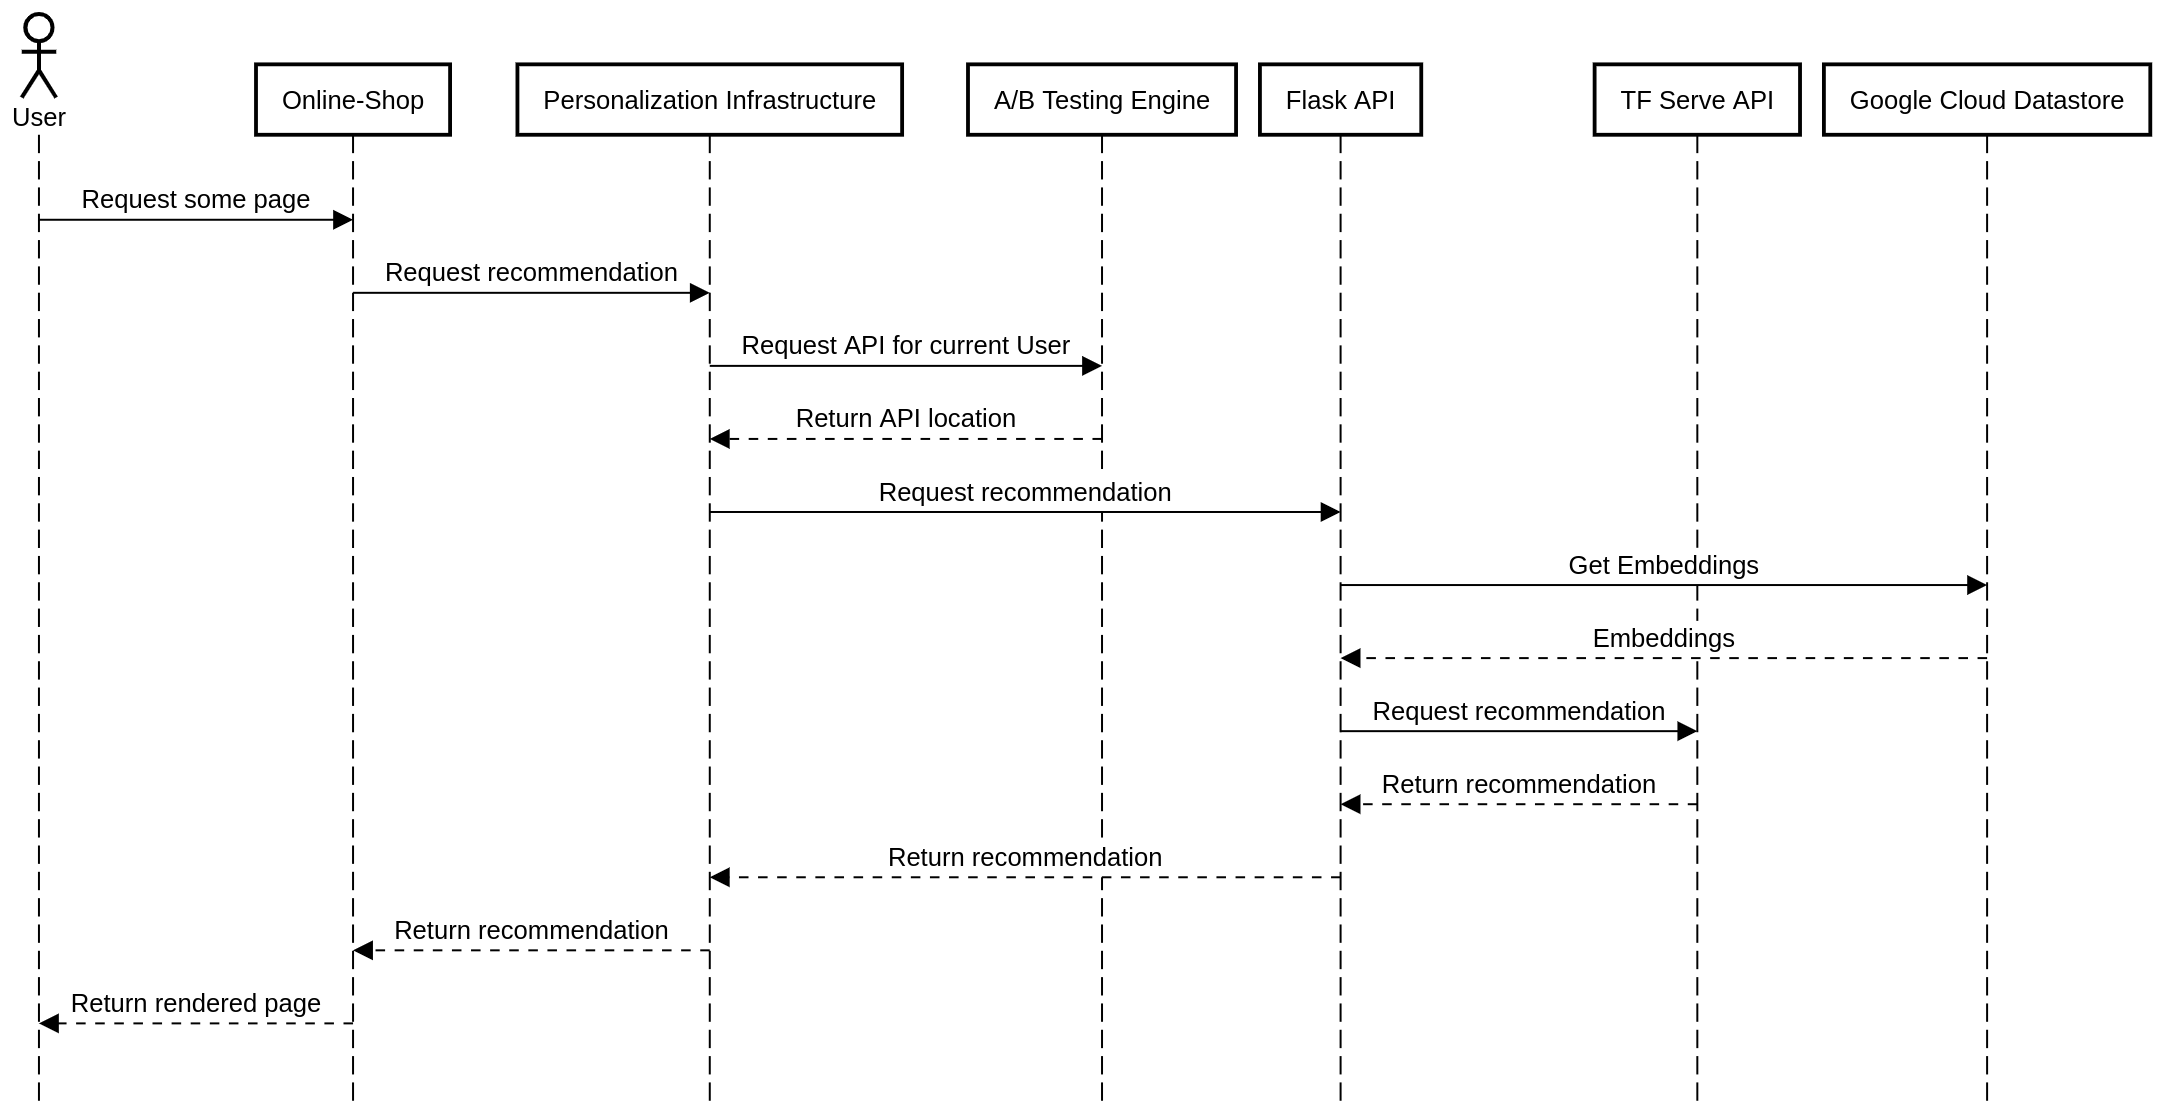
\includegraphics[width=\textwidth]{serving-recommendations.png}
    \caption{Serving Recommendations on digitec.ch and galaxus.ch}
    \label{fig:serving_recs}
\end{figure}

The whole process starts when a specific user requests a specific page on either digitec.ch or galaxus.ch.
If the requested page has an element where there is an A/B test configured the Online-Shop Application will make a request to the testing engine.
As mentioned above the testing engine will then make a request to a API location, which corresponds to one of the model versions.
After that the Online Shop will request the content, in this case, from the Personalization Infrastructure.
Note that during this setup each of the four versions of the model is deployed simultaneously, all of them trained on the same dataset.
The Personalization Infrastructure then calls the API described above.
Before requesting a prediction from tf-serve the API will gather precomputed embeddings for the involved entities.
The predictions are returned to the Personalization Infrastructure and from there to the Online Shop.
The last step is for the Online Shop to render the content and deliver the page to the user.
This process takes about XXms\todo{Get ms number here}ms.
\chapter{Experiments}
The models described in section~\ref{sec:model_arch} are all tested in two test scenarios.
The offline test scenario measures the performance of the model on historical data, whereas the online scenario measures KPIs in a production setting on new data.
The reasoning behind this is that when using recommendation systems and evaluating them on historical data, the results do not necessarily reflect the real life behaviour of users.
This is because displaying recommendations changes the reality, i.e. what the user sees when using the application is different from what the user saw in the past without or with other recommendation systems.
\section{Offline}
\subsection{Experiment Setup}\label{sec:exp_setup}
In this scenario we do a temporal split and hold off future data for evaluation and train the model on historical data.
That means that the most recent sessions of each user make up the test set, while the second most recent sessions of each user make up the validation set.
Each model is evaluated on the validation set regurarly during training.
The goal of this experiment is to predict the next click of the user, given the currently active product.
After completing the training, i.e. after the validation metric does not increase anymore, the model is evaluated on the test set.
Before running the model on the MAXI dataset, some parameters were chosen based on experiments on the MIDI dataset, since due to time and resource constraints it was not possible to train all combinations of the models on the MAXI dataset.
Specifically the loss function, optimizer, batch size, learning rate, gradient clipping threshold and early stopping criterion were chosen based on the MIDI dataset, since as mentioned before it was not possible to test all these different configurations on the large dataset.
Further the one-hot encoding variants used so much time and resources, only the best performing models on the MIDI dataset were trained on the MAXI dataset.
Finally the models that used the product embedding trained much faster, therefore there were multiple versions tested for the MAXI dataset.
\par
For each model we measured two metrics of the validation set, since each of the metrics measures a different aspect of the performance of the model.
Specifically Recall@10 was measured to determine in how many cases the top 10 recommended products contained the product that was actually clicked by the user.
MRR@10 was measured to determine where the product was ranked in the top 10 predictions.
A perfect model would achieve a value of 1 in both metrics, i.e. the next clicked product is always the top prediction.
However while MRR@10 is the more informative metrics of the two, giving insight in the ranking of "good" predictions, Recall@10 is the more important one.
Achieving a Recall@10 of 1 means the next clicked item is always in the top 10 predictions, which means the user will see the recommendation, whether it is the top prediction or the fifth, which essentially is the goal of this task.
\subsection{Measurements}

\begin{table}[t]
    \centering
    \begin{tabular}{|c|c|c|c|c|}
        \hline
        User Layer & Loss Function & RNN Units & MRR@10 & Recall@10 \\ \hline
        yes & Top 1 & 50 & ?? & ??\todo{Get number when model is finished} \\ \hline
        yes & Cross Entropy & 100 & 0.058 & 0.167 \\ \hline
        yes & Top 1 & 100 & 0.099 & 0.226 \\ \hline
        yes & Top 1 & 250 & 0.073 & 0.167\todo{Verify number from most recent run} \\ \hline
        no & Top 1 & 50 & ?? & ??\todo{Get number when model is finished} \\ \hline
        no & Cross Entropy & 100 & 0.069 & 0.193 \\ \hline
        no & Top 1 & 100 & 0.112 & 0.258 \\ \hline
        no & Top 1 & 250 & 0.121 & 0.278 \\ \hline
    \end{tabular}
    \caption{Measurements on MIDI Dataset (One-Hot)}
    \label{tab:midi_dataset_measurements}
\end{table}

The measurements on the MIDI dataset are summarized in table~\ref{tab:midi_dataset_measurements}.
As mentioned above these are all measurements from the models using the one-hot encoding as input.
As can be seen the Top 1 loss introduced by the authors of~\cite{gru4rec} performs better than the cross entropy loss.
This is because the cross entropy loss essentially compares the probabilities that are predicted by the model with the "real" probability distribution, in this case with the one-hot encoding of the label.
In contrast the Top 1 loss is a strict ranking loss, only concerned with the position of the label in the predictions, which better models the task of recommendation.
Further it can be seen that the improvement of using 250 units per GRU instead of 100 is marginal, therefore larger models were not tested.
Therefore the models using 250 units per GRU were chosen to be trained on the MAXI dataset in addition to the ones using the product embedding.
Finally it can be seen that the models using the user level GRU perform approximately the same, sometimes even worse than the models using only the session level GRU, the reason for this will be discussed in the next chapter.
\begin{table}[t]
    \centering
    \begin{tabular}{|c|c|c|c|c|}
        \hline
        User Layer & RNN Units & MRR@10 & Recall@10 \\ \hline
        yes & 250 & 0.055 & 0.138 \\ \hline
        no & 250 & 0.061 & 0.146 \\ \hline
    \end{tabular}
    \caption{Measurements on MAXI Dataset (One-Hot)}
    \label{tab:maxi_dataset_measurements_one_hot}
\end{table}
The measurements for the models using the one-hot on the MAXI dataset are summarized in table~\ref{tab:maxi_dataset_measurements_one_hot}.
There is nothing surprising here, again we can see that the user-level GRU apparently does not help the performance of this task.

\begin{table}[t]
    \centering
    \begin{tabular}{|c|c|c|c|c|}
        \hline
        User Layer & RNN Units & MRR@10 & Recall@10 \\ \hline
        no & 25 & 0.012 & 0.025 \\ \hline
        no & 50 & 0.011 & 0.22 \\ \hline
        no & 100 & 0.012 & 0.025 \\ \hline
        no & 250 & diverged & diverged \\ \hline
        yes & 25 & 0.013 & 0.22 \\ \hline
        yes & 50 & 0.011 & 0.023 \\ \hline
        yes & 100 & 0.11 & 0.023 \\ \hline
        yes & 250 & diverged & diverged \\ \hline
    \end{tabular}
    \caption{Measurements on MAXI Dataset (Embedding)}
    \label{tab:maxi_dataset_measurements_embedding}
\end{table}
In the table~\ref{tab:maxi_dataset_measurements_embedding} the measurements for the models using the product embedding on the MAXI dataset are summarized.
As can be quickly seen the models do not perform nearly as well as the models using the one-hot encoding.
Further the model does not improve when increasing the model size, which indicates that this is due to the product embeddings.
Also this will be a topic explored in detail in the next chapter.
\section{Online Experiment Setup}
\subsection{Experiment Setup}
In this scenario we train the models on all the available data and evaluate the performance on live data generated by users that use the web application.
For this we chose the best performing configuration for each variant (c.f.~\ref{tab:model_archs}) from the offline experiments.
Using these four models an A/B/C/D/E test was setup.
An A/B/n test is often used when testing features for online services.
Such a test consists of choosing different versions of the same element or feature and then partition the traffic into groups, where each group is assigned to one version of the element.
One of the versions should always serve as a control group, receiving the original version of the element.
The user to group assignment is done at random to get evenly distributed groups.
This group assigment is also persistent across different sessions.
After such a test is setup, the test is run for some time while measuring KPIs per group.
Then after ending the test the best performing version can be chosen based on the KPIs measured during the test.
\par
The element that was tested in this work is the first slot for recommendations on the product detail page, the page that receives the most traffic.
The slot is illustrated in figure~\ref{fig:ab_test_slot}.
\begin{figure}[t]
	\centering
	\captionsetup{width=0.8\textwidth}
    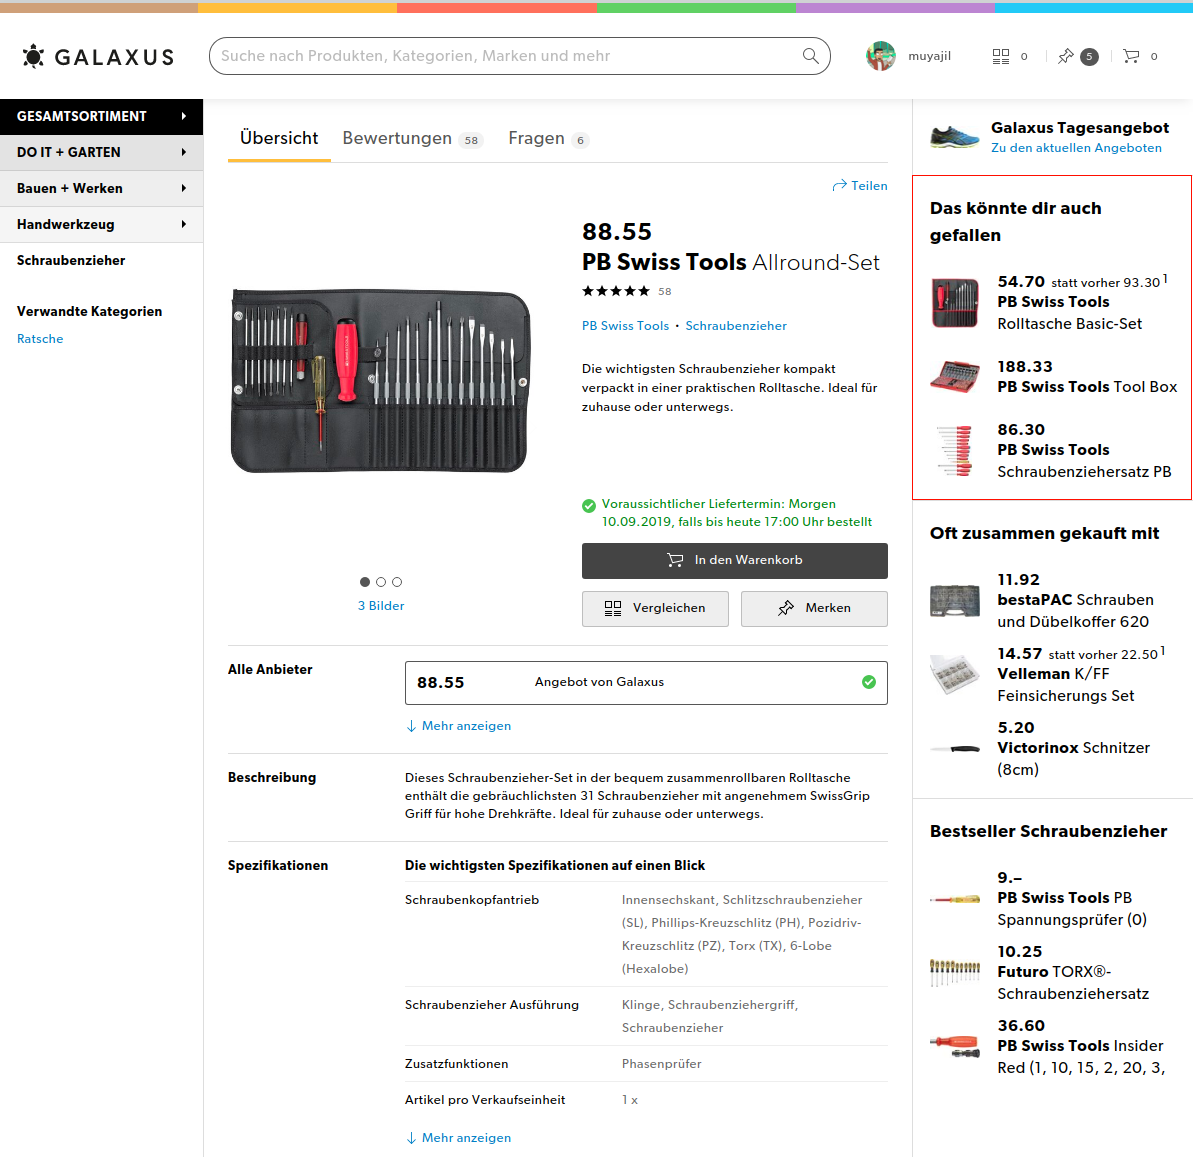
\includegraphics[width=\textwidth]{ab_test_slot.png}
    \caption{Recommendation slot on the product detail page}
    \label{fig:ab_test_slot}
\end{figure}
As a control version a black-box recommendation system provided by Google called Recommendations AI~\footnote{\url{https://cloud.google.com/recommendations/}} was chosen.
In the normal mode the chosen recommendation slot still has multiple recommendation engines which can be chosen according to a framework, however Recommendations AI is the best performing one.
Other than the logic chooses the products to display nothing was changed, i.e. the title and design remained identical.
The test was run for 14 days to reflect one whole business cycle.
\par
Something important to note at this stage is the postprocessing of recommendations coming either from the tested model or Recommendations AI.
There are some constraints that are applied on the recommended product, such as filtering products that are inappropriate (e.g. alcoholic beverages, erotic articles etc.) and products that are not available for sale anymore (e.g. discontinued products, not on stock).
This post processing is applied on all recommendation engines, therefore still providing a leveled playing field.
However this is one of the reasons why production testing makes sense for recommendation systems, since this can never be reproduced in an offline setting, since some of these factors change over time.
\subsection{Measurements}
In table~\ref{tab:online_measurements} we can see the measurements for the different variants of the model in the online setting, as well as the same metric for different models that have been displayed in the same slot as the one we tested in.
We focus on the Click-Through rate in this experiment, since as mentioned before the conversion rate is difficult to compute, and due to time constraints we could not wait 14 days after the test was finished to get a good estimation of this metric.
The test was executed on approximately 1.3 Million sessions.
The metrics for each of the recommendation engines is averaged over all the sessions.
\begin{table}[t]
    \centering
    \begin{tabular}{|c|c|}
        \hline
        Model Name & CTR \\ \hline
        OnlySessionOneHot & 2.1\% \\ \hline
        OnlySessionEmbedding & 0.85\% \\ \hline
        WithUserOneHot & 2\% \\ \hline
        WithUserEmbedding & 0.9\% \\ \hline
        Recommendations AI & 5.55\% \\ \hline
        Often Bought Together & 0.91\% \\ \hline
        Similar Products & 1.19\% \\ \hline
    \end{tabular}
    \caption{Measurements on Live Data}
    \label{tab:online_measurements}
\end{table}
Often Bought Together is a simple model counting which products are bought with which other products.
It is very similar to the one described in section~\ref{sec:often_bought_together}.
Similar Products is a recommendation engine also using the product embeddings produced by Meta-Prod2Vec.
This engine will recommend the items that are closest to the currently active item in the embedding space.
\par
As can be seen in table~\ref{tab:online_measurements} nothing comes close to achieving the same result as Recommendations AI.
This is a proprietary system which is acessed directly via an API, however the data that is ingested by this system is very diverse.
The system does not only consider the currently viewed item and the active user, but also takes into account trends, recent sales and a lot of other information.
However when compared to more classical approaches the session-based approach performs much better, at least when using the one-hot encoding, since also in this setting we can see that the models using the product embedding perform much worse.

\chapter{Results}
The goal of this thesis was to improve the session-based recommendation system using product embeddings.
From the previous chapter it is clear that this approach did not work as intended.
There are mainly two interesting things about the measurements in the experiments.
First the user-layer does not seem to improve the performance, depending on the configuration even produces worse results than unpersonalized session-based recommendations.
The authors of~\cite{hierarchical} found that the performance of the model depends strongly on the user history length.
However in their case the user-level GRU still improves the performance, even for short user histories.
The main difference between the datasets used in~\cite{hierarchical} and the datasets used in this work, is the distribution of the lengths of the sessions.
The datasets in~\cite{hierarchical} in general have less sessions that are longer.
If we look at the type of datasets used this makes sense.
In~\cite{hierarchical} the authors used two datasets, one dataset comes from XING, an social network for professionals similar to LinkedIn, the second dataset is from a proprietary video platform similar to YouTube.
The fundamental difference between the afromentioned dataset and the one used in this work is the possible entrypoints to the services.
Both, XING and the video platform, offer a service which is sort of self-contained.
On both services the user is served with everything that is needed in the same platform, searching for jobs, connecting with colleagues etc. can all be done in the same session.
For an online-store this is a bit different.
Many users use other entrypoints to the online-store, such as Google searches, Ads or price comparison pages.
A bounce rate analysis shows, that 46\% of users arriving on the product detail page, leave the site without accessing any other pages on the platform, i.e. the users use the online-store for researching product information, but not for browsing.
Each of these visits still produced a session, this would explain the shorter sessions in our dataset. 
Of course it is clear that even when identifying the user, by looking at one product there is not much information to carry over to the next session.
Another issue is that there are very many users which do have very few sessions. 
\begin{figure}[t]
	\centering
	\captionsetup{width=0.8\textwidth}
    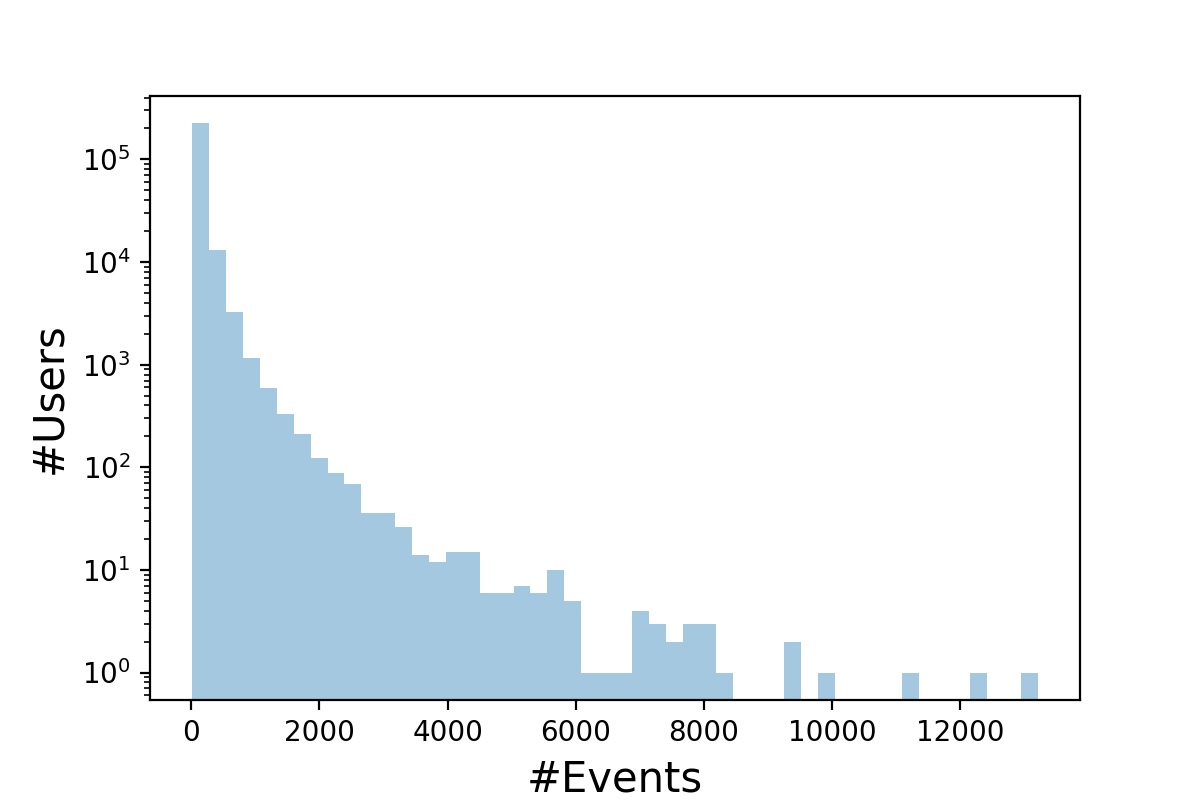
\includegraphics[width=\textwidth]{histo_user_visits.png}
    \caption{Distribution of the number of visits per user (log-scale)}
    \label{fig:histo_user_events}
\end{figure}
If we look at figure~\ref{fig:histo_user_events} we can see the distribution of the number of visits per user.
What can be seen in the histogram is a phenomenon called \emph{the Long Tail} in the context of web analytics.
There is a very high proportion of the users which produce very little datapoints, at the same time there is a very long tail in the distribution, where some users produce extremely many events.
Thus the information that can be extracted from the majority of users is rather limited.
Of the approximately 250K users there are about 170K users that produced at most 100 events in total across all sessions.
This would explain the limited amount of cross session information we can learn when adding the user-level GRU.
Because of that the user embedding will not change much from its initial random intitialization, effectively changing nothing about the model, since without the user layer a session would be initialized at random as well.
\par
The second thing is that the product embedding greatly worsens the results in the offline as well as the online setting.
The reason for this is similar as explained above.
\begin{figure}[t]
	\centering
	\captionsetup{width=0.8\textwidth}
    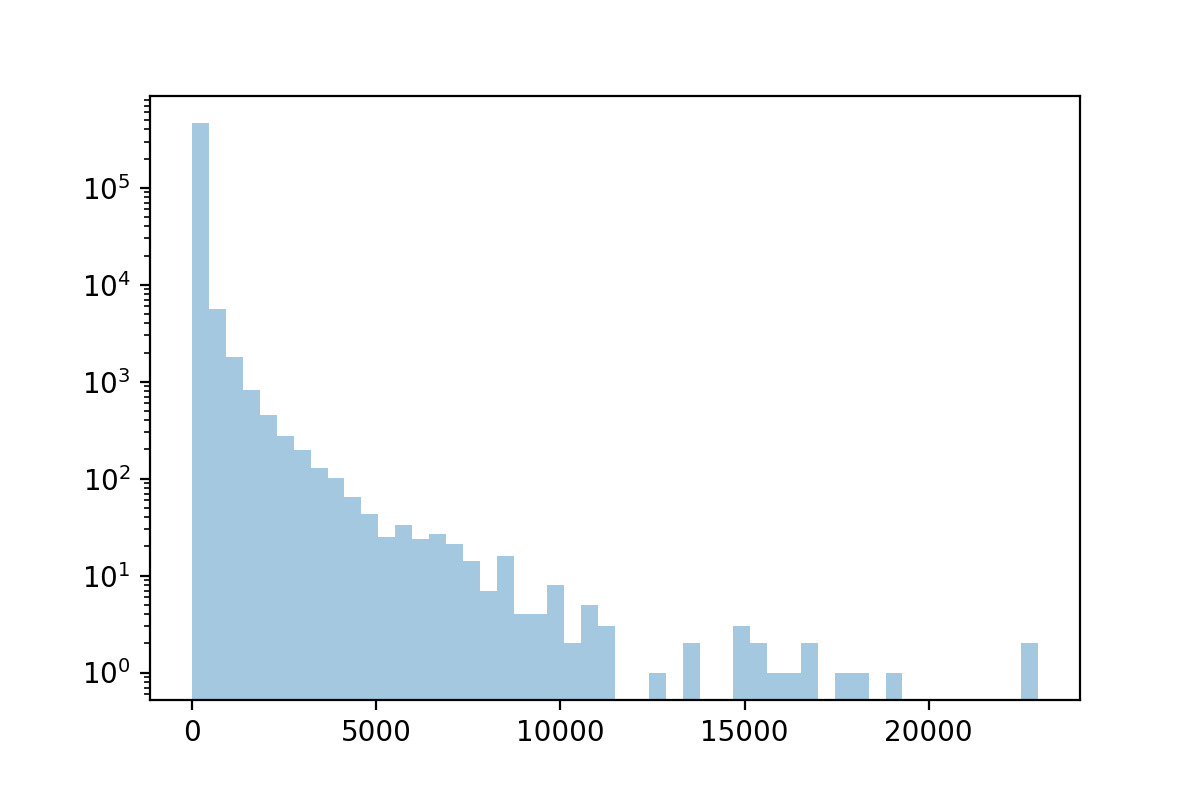
\includegraphics[width=\textwidth]{histo_product_visits.png}
    \caption{Distribution of the number of visits per product (log-scale)}
    \label{fig:histo_product_events}
\end{figure}
In figure~\ref{fig:histo_product_events} we can see the same long tail effect as with the users.
Of the approximately 470K products about 320K have at most 100 events recorded.
\begin{figure}[t]
	\centering
	\captionsetup{width=0.8\textwidth}
    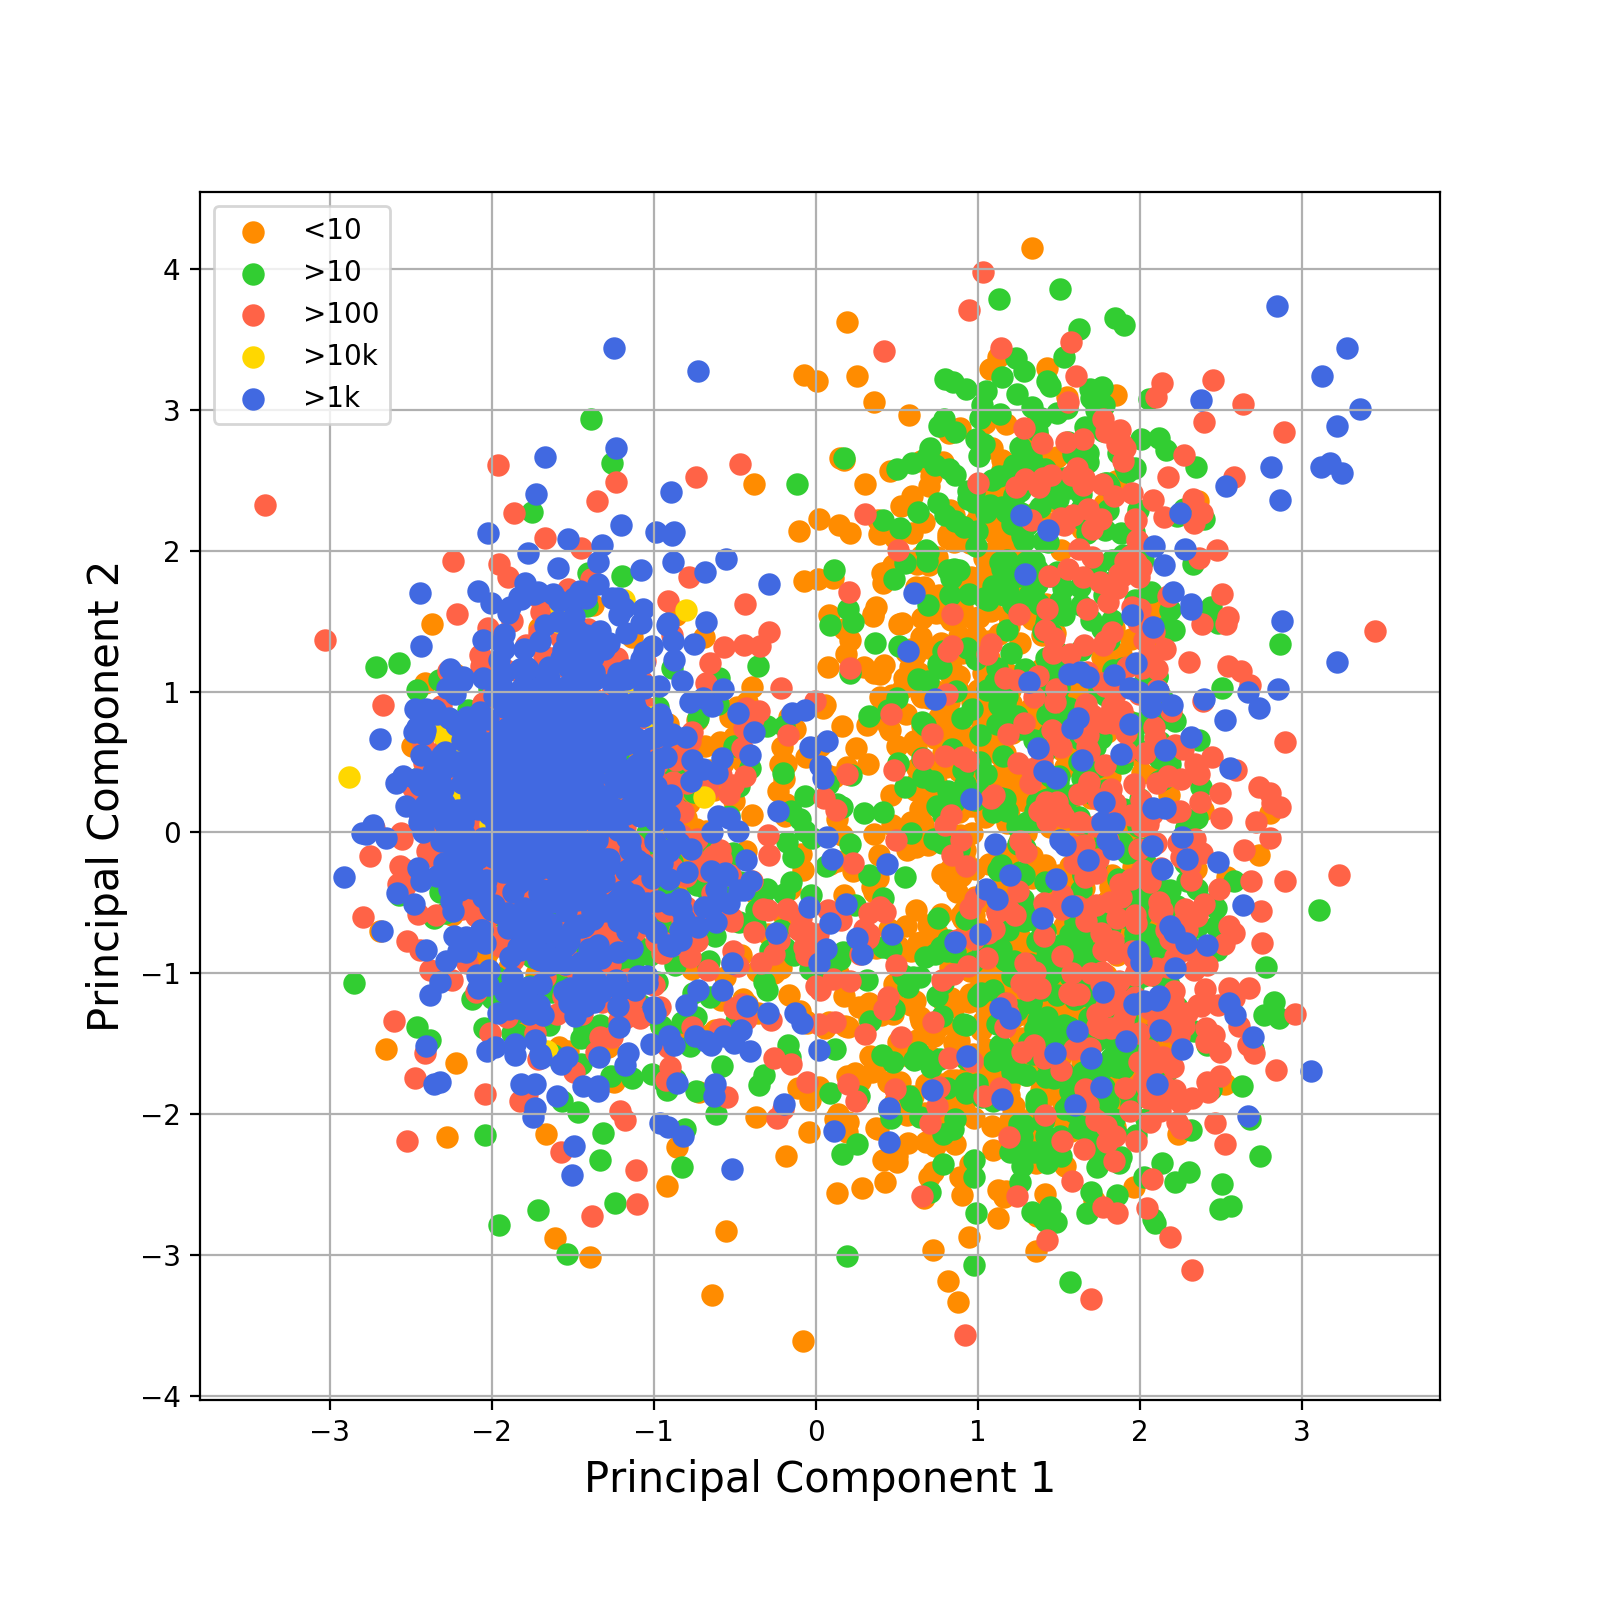
\includegraphics[width=\textwidth]{products_pca.png}
    \caption{PCA of product embeddings}
    \label{fig:products_pca}
\end{figure}
In figure~\ref{fig:products_pca} we can see a PCA analysis of the product embeddings.
As can be seen in the PCA there is a separation of datapoints in the first principal component.
\begin{figure}[t]
	\centering
	\captionsetup{width=0.8\textwidth}
    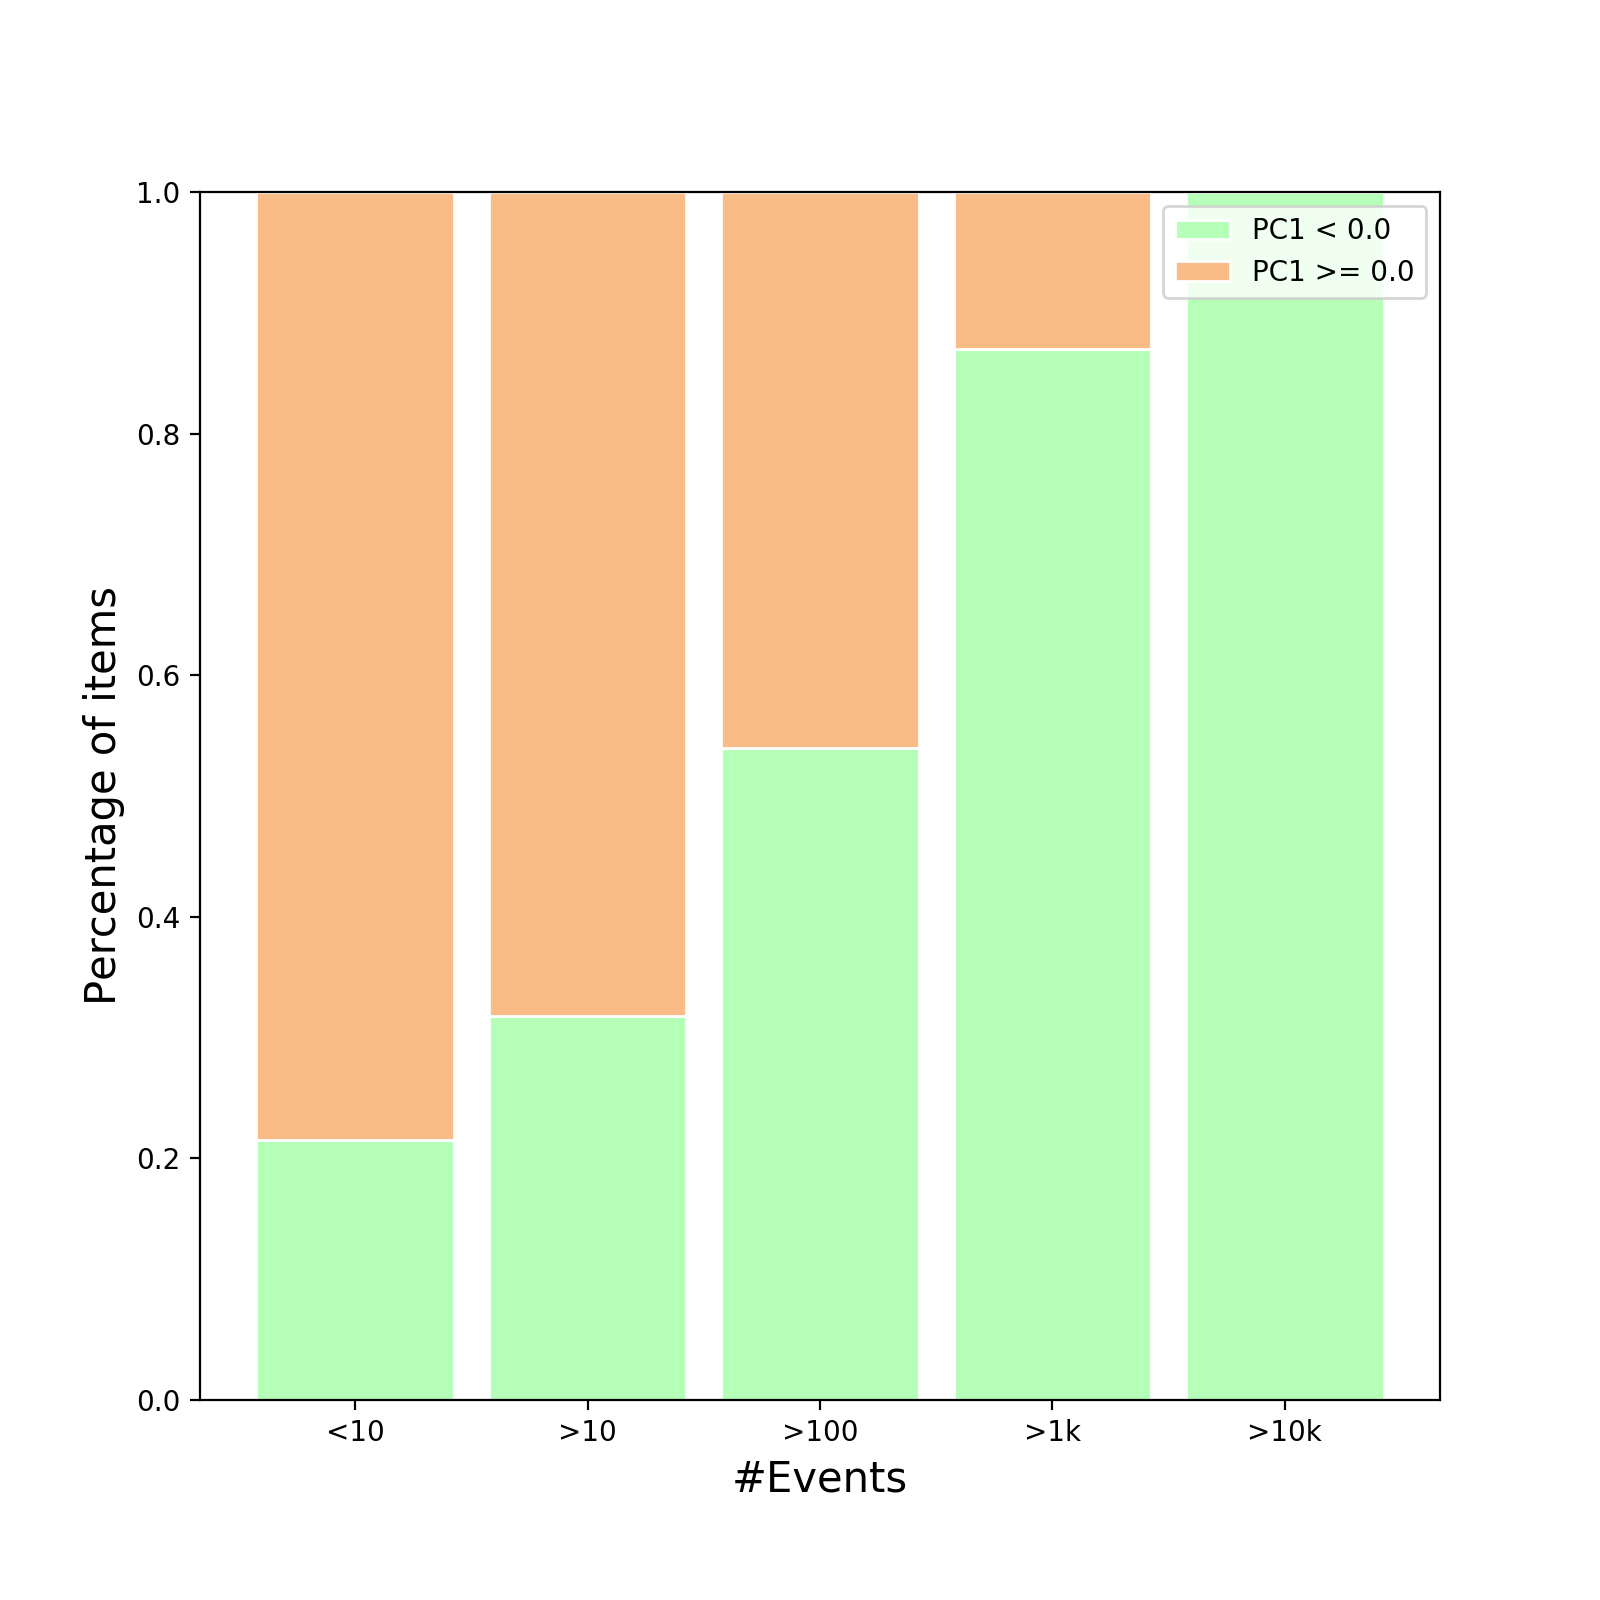
\includegraphics[width=\textwidth]{products_pca_groups.png}
    \caption{Value of PC1}
    \label{fig:products_pca_groups}
\end{figure}
In figure~\ref{fig:products_pca_groups} we can see the percentage of datapoints that have the first principal component smaller than 0, grouped by the number of events per product.
It is clear from this that the products that generate a lot of events can clearly be separated from the ones producing few events.
That means again that the majority of the product embeddings does not move much from the initial random initialization, since the majority of the products have less than 100 events.
Therefore it can happen that for example a dining table with very few visits is very similar to a shoe with few visits, since both vectors are initialized uniformly at random drawing values from the same distribution.
The problem with this is the signal that is propagated to the GRU.
When using the one-hot encoding there is always a clear signal which product was the one that was viewed, with the product embedding this is not the case.
Therefore the network in many cases, basically receives random noise as an input, not being able to produce something else in the output layer.
This has the effect that the predictions in the models using the product embeddings are almost always the same, recommending items that are viewed many times, but do not have much relation to the currently active item.
\par
In conclusion it can be said that the sesssion-based approach clearly works, even if it does not match the performance of a commercial product, it performs better than more classical approaches to recommendation.
However personalizing these recommendations turns out to be more difficult than initially thought.
It greatly depends on the number of events produced by each user.
Therefore it might make sense to focus on personalizing the experience for the subset of users that actually produce enough events.
The same can be said for the introduction of product embeddings, the product embeddings have to be very good such that the network can interpret the signal correctly.
At least the properties of the dataset have a very large influence on the success of both the personalization of the recommendations as well as the usage of product embeddings.
\par
A future improvement of this work would be the use of transfer learning.
If the currently active item is an item with very few events, a similar item with more events can be used as a replacement as a basis for the recommendation.
However this would require a secondary similarity measure.
It would also be useful to improve the product embedding, in~\cite{content2vec} a model is introduced which, in addition to meta information also takes into account images of a product and its textual description.
Another approach to improving the product embedding could be to parametrize the distribution for the initialization of the vectors to some side-information.
This would at least remove the issue that very dissimilar products have close embeddings.
Finally another improvement that could be explored is to not only model the sequence of product detail pages, but all the different types of pages in such an online-store.
This would give the system the ability to recommend review articles or categories for the user to explore.

% \appendix

% \chapter{Dummy Appendix}

You can defer lengthy calculations that would otherwise only interrupt
the flow of your thesis to an appendix.


\backmatter

\bibliographystyle{plain}
\bibliography{refs}

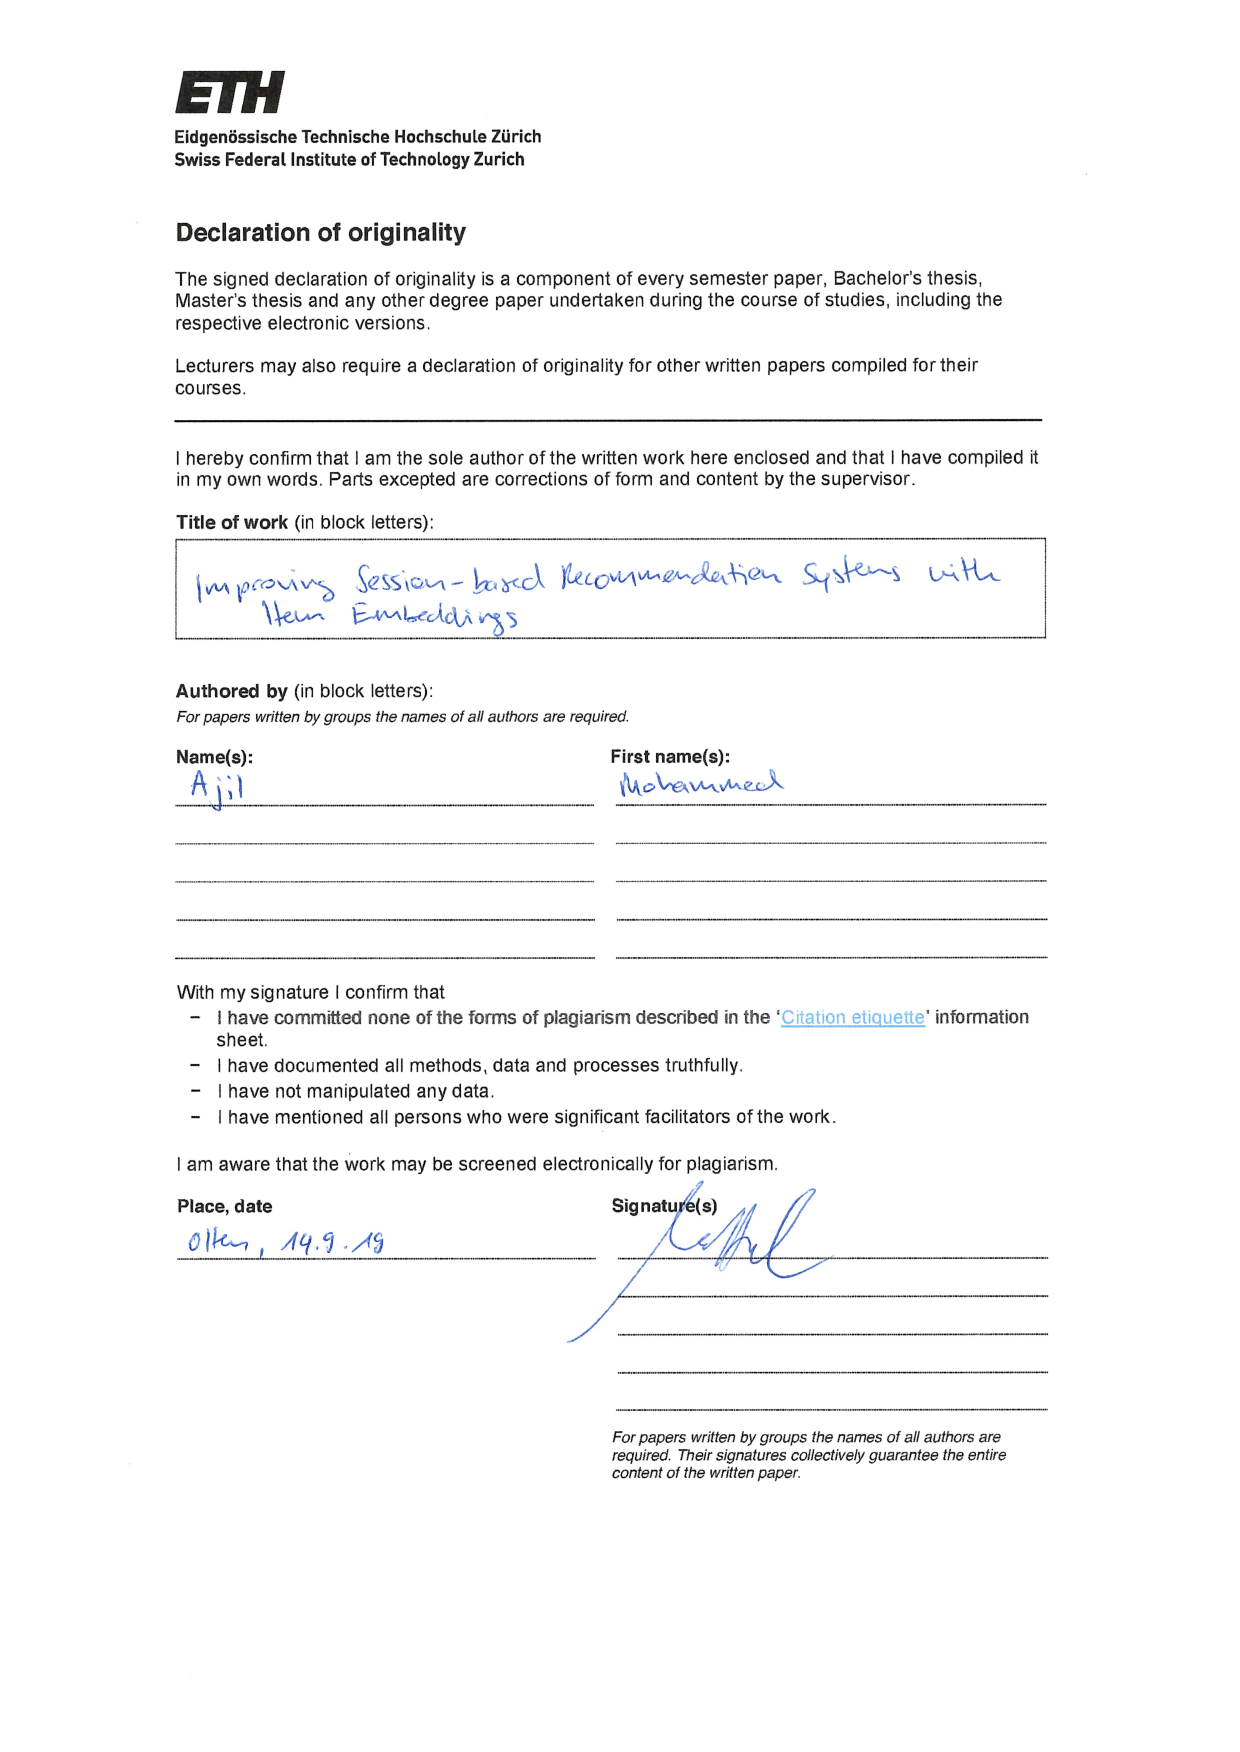
\includepdf[pages={-}]{declaration-originality.pdf}

\end{document}
